\documentclass[12pt]{exam}
\usepackage[utf8]{inputenc}
\usepackage{amsmath,amstext,amsthm,amssymb,amsxtra, graphicx}
\usepackage[top=1.5in, bottom=1.5in, left=1.25in, right=1.25in]	{geometry}
%\usepackage[normalem]{ulem}
\usepackage{txfonts} % pxfonts txfonts 
\usepackage[T1]{fontenc}
\usepackage{lmodern}
\renewcommand*\familydefault{\sfdefault}
 \usepackage{euler}   % better than the option below
\usepackage{pdfsync}
\usepackage{multicol}
\newcommand{\ci}[1]{_{ {}_{\scriptstyle #1}}}
\graphicspath{ {images/} }


\newcommand{\norm}[1]{\ensuremath{\left\|#1\right\|}}
\newcommand{\abs}[1]{\ensuremath{\left\vert#1\right\vert}}
\newcommand{\ip}[2]{\ensuremath{\left\langle#1,#2\right\rangle}}
\newcommand{\p}{\ensuremath{\partial}}
\newcommand{\pr}{\mathcal{P}}

\newcommand{\pbar}{\ensuremath{\bar{\partial}}}
\newcommand{\db}{\overline\partial}
\newcommand{\D}{\mathbb{D}}
\newcommand{\B}{\mathbb{B}}
\newcommand{\Sp}{\mathbb{S}}
\newcommand{\T}{\mathbb{T}}
\newcommand{\R}{\mathbb{R}}
\newcommand{\Z}{\mathbb{Z}}
\newcommand{\C}{\mathbb{C}}
\newcommand{\N}{\mathbb{N}}
\newcommand{\Q}{\mathbb{Q}}
\newcommand{\mQ}{\mathcal{Q}}
\newcommand{\mS}{\mathcal{S}}
\newcommand{\scrH}{\mathcal{H}}
\newcommand{\scrL}{\mathcal{L}}
\newcommand{\td}{\widetilde\Delta}
\newcommand{\pw}{\text{PW}}
\newcommand{\esup}{\text{ess.sup}}
\newcommand{\Tn}{\mathcal{T}_n}
\newcommand{\Bn}{\mathbb{B}_n}
\newcommand{\rt}{\mathcal{O}}
\newcommand{\avg}[1]{\langle #1 \rangle}
\newcommand{\one}{\mathbbm{1}}
\newcommand{\eps}{\varepsilon}
\newcommand{\grad}{\nabla}

\newcommand{\La}{\langle }
\newcommand{\Ra}{\rangle }
\newcommand{\rk}{\operatorname{rk}}
\newcommand{\card}{\operatorname{card}}
\newcommand{\ran}{\operatorname{Ran}}
\newcommand{\osc}{\operatorname{OSC}}
\newcommand{\im}{\operatorname{Im}}
\newcommand{\re}{\operatorname{Re}}
\newcommand{\tr}{\operatorname{tr}}
\newcommand{\vf}{\varphi}
\newcommand{\f}[2]{\ensuremath{\frac{#1}{#2}}}

\newcommand{\kzp}{k_z^{(p,\alpha)}}
\newcommand{\klp}{k_{\lambda_i}^{(p,\alpha)}}
\newcommand{\TTp}{\mathcal{T}_p}
\newcommand{\m}[1]{\mathcal{#1}}
\newcommand{\md}{\mathcal{D}}
\newcommand{\qan}{\abs{Q}^{\alpha/n}}
\newcommand{\sbump}[2]{[[ #1,#2 ]]}
\newcommand{\mbump}[2]{\lceil #1,#2 \rceil}
\newcommand{\cbump}[2]{\lfloor #1,#2 \rfloor}

\newcommand{\hn}{{1}}
\newcommand{\dd}{{09-07}}
\newcommand{\class}{Aero 417}
\newcommand{\term}{Fall 2024}
\newcommand{\examnum}{Homework \hn: Due \dd}
\newcommand{\examdate}{}
\newcommand{\timelimit}{75 Minutes}
\newcommand{\vc}[3]{\langle #1,#2,#3\rangle}
\newcommand*{\vv}[1]{\vec{\mkern0mu#1}}
\newcommand{\bv}[1]{\boldsymbol{#1}}
\newcommand{\hide}[1]{}
\newcommand{\uvec}[1]{\boldsymbol{\hat{\textbf{#1}}}}
\newcommand{\vex}[1]{\boldsymbol{{\textbf{#1}}}}
\newcommand{\px}{\frac{\partial}{\partial x}}
\newcommand{\py}{\frac{\partial}{\partial y}}
\newcommand{\pt}{\frac{\partial}{\partial t}}
\newcommand{\pxx}{\frac{\partial^2}{\partial x^2}}
\newcommand{\pyy}{\frac{\partial^2}{\partial y^2}}
\newcommand{\ptt}{\frac{\partial^2}{\partial t^2}}


\pagestyle{head}
\firstpageheader{}{}{}
\runningheader{\class}{ Page \thepage\ of \numpages}{\examnum}
\runningheadrule

\makeatletter
\renewcommand*\env@matrix[1][*\c@MaxMatrixCols c]{%
  \hskip -\arraycolsep
  \let\@ifnextchar\new@ifnextchar
  \array{#1}}
\makeatother

%\printanswers
\begin{document}

\noindent
\begin{tabular*}{\textwidth}{l @{\extracolsep{\fill}} r @{\extracolsep{6pt}} l}
\textbf{\class} & \textbf{Name:} & \makebox[2in]{\bf{Benjamin Tollison}}\\
\end{tabular*}\\
\rule[2ex]{\textwidth}{2pt}
%
\begin{questions}
\begin{question}
Create a graphic in a spreadsheet, showing the variaon of the normalized specific work
vs pressure rao (r) for different t values (1, 2, 3, 4, and 5). Explain the behavior of the
curves based on the technological level of metals. Use: \(\gamma\) = 1.4 (air).
\[\frac{W_L}{c_p T_{t1}} = t \left[1-\frac{1}{r^{\frac{\gamma-1}{\gamma}}}\right] - \left[r^{\frac{\gamma-1}{\gamma}} -1\right]\]
\end{question}
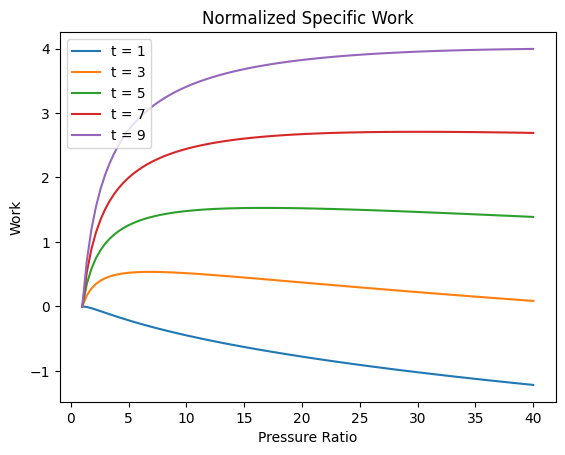
\includegraphics[width=\linewidth]{Hw1-1-graph.png}

\newpage 
\begin{question}
About the text: for a Brayton Cycle, the maximum normalized specific work is obtained
when \(T_2 = T_4\) (compressor outlet temperature = turbine outlet temperature). Is this true
or false? 
\end{question}
\begin{equation}
  \frac{W_L}{c_p T_{t1}} = t \left[1-\frac{1}{r^{\frac{\gamma-1}{\gamma}}}\right] - \left[r^{\frac{\gamma-1}{\gamma}} -1\right]
\end{equation}
\begin{equation*}
  \text{Where: } t = \frac{T_{t3}}{T_{t1}}, r^{\frac{\gamma-1}{\gamma}} = \frac{T_{t2}}{T_{t1}} = \frac{T_{t3}}{T_{t4}}
\end{equation*}
\begin{equation}
  \frac{W_L}{c_p T_{t1}} = \frac{T_{t3}}{T_{t1}} \left[1-\frac{T_{t1}}{T_{t2}}\right] - \left[\frac{T_{t2}}{T_{t1}} -1\right]
\end{equation}


\end{questions}
\end{document}